% \numberwithin{equation}{section}

\chapter{Introducció} \label{sec:intro}


%\sloppy - %\begin{flushleft}
% És una bona alternativa per separar explícitament paràgrafs, però ja està solventat amb el parskip de l'inici.
%\fussy - %\end{flushleft}

Les estrelles conformen pràcticament la totalitat de la massa bariònica de l'univers i es troben en un estat de la matèria anomenat plasma.
Aquest consisteix en un gas ionitzat on els àtoms i els ions es poden moure lliurement, així com els electrons.
Amb aquestes condicions es dedueix que el plasma és un bon conductor elèctric i altament sensible a camps magnètics.
Per tant, en presència d'un camp magnètic les equacions que descriuen el seu comportament són les de la magnetohidrodinàmica (MHD).

El Sol és una estrella de la seqüència principal de tipus espectral G2V.
El camp magnètic de la seva atmosfera interacciona fortament amb el plasma, de manera que es generen taques solars, flamarades, protuberàncies, bucles coronals, etc.
L'objecte d'aquest estudi són les protuberàncies solars,
objectes pesats que es mantenen suspesos pel camp magnètic per damunt de la superfície solar dins la corona,
la part més externa i calenta de l'atmosfera solar.

La temperatura de la corona és molt elevada ($\sim 10^6$~K) i la densitat molt baixa ($\sim 10^{12}$~m$^{-3}$) respecte altres punts de l'atmosfera com la fotosfera o la cromosfera.
En canvi, una protuberància presenta una densitat major ($10^{15}-10^{17}$~m$^{-3}$) i una temperatura molt menor ($\lesssim10^4$~K) que la de la corona que l'envolta.


El fi d'aquest treball és l'estudi de la propagació d'ones lineals sobre l'estat quiescent d'una protuberància dins la corona solar mitjançant l'ús de Dedalus \parencite{Dedalus},
una llibreria de Python enfocada a resoldre equacions diferencials parcials (PDE per les seves sigles en anglès) com les MHD.
El funcionament de Dedalus consisteix principalment en transformar la informació de l'espai real a l'espai de Fourier,
realitzar els càlculs necessaris i retornar a l'espai real.

El camp de les ones en estats quiescents de protuberàncies solars ha estat estudiat intensivament per la comunitat científica.
Un dels llibres més important de física solar va ser escrit en els anys 80 per \textcite{Priest_2014}.
Els fonaments d'aquest estudi es troben en els Caps.~1,~2,~4~i~11 d'aquest,
juntament amb els articles de \textcite{oscillation_modes_II} i d'\textcite{oscillations_quiescent_solar_prominence},
que consideren una estructura simplificada per representar una protuberància en la corona solar.


%---------------------------------------------------------------------------------------------------------------------------------------------------
% OJO AMB PEGAR-TE UN TIR AL PEU
%---------------------------------------------------------------------------------------------------------------------------------------------------

%Les protuberàncies es formen a partir de la reconnexió del camp magnètic en les zones d'inversió de polaritat o a partir de la interacció de dos sistemes de flux de camp magnètic.
%Per aquest motiu, moltes protuberàncies presenten una polaritat invertida.
%Aquests processos fan ascendir la gran massa que conforma la prominència de la cromosfera o de la fotosfera, capes atmosfèriques inferiors a la corona.

%Les prominències generades en zones actives són menors en tamany i més denses que les quiescients, que són generades enfora de les zones d'alta activitat solar.
%Aquelles que es formen en el límit d'una zona activa s'anomenen protuberàncies intermitges.

El camp magnètic és pràcticament horitzontal en les protuberàncies quiescents, com es pot apreciar en la Fig.~\ref{fig:prot_real}.
Aquesta es basa en Fig.~11.1 del llibre de \textcite{Priest_2014}.
La manera d'esquematitzar la protuberància solar consisteix en suposar-la com una llosa o làmina plana.

A més, s'imposa la condició de camp magnètic estrictament constant en mòdul i direcció.
La manera d'aconseguir aquest sistema és situar la superfície com a doble condició de contorn, als extrems.
Com que es tracta de la superfície, les velocitats als extrems són nul·les, perquè quan una pertorbació que viatja dins la corona impacta contra la fotosfera,
aquesta no es veu afectada degut a que és molt més densa que la corona, per on viatja l'ona.
En conseqüència, apareixen modes normals fortament dependents de la regió central, la protuberància.

Finalment el sistema resulta com en la Fig.~\ref{fig:sistema}. Aquesta representació es basa en la Fig.~1 de l'article \textcite{oscillation_modes_II}.
Per veure una imatge real d'una protuberància solar es pot consultar l'apèndix~\ref{ap.C}.
\begin{figure}[H]
    \centering
    \begin{subfigure}{0.48\textwidth}
        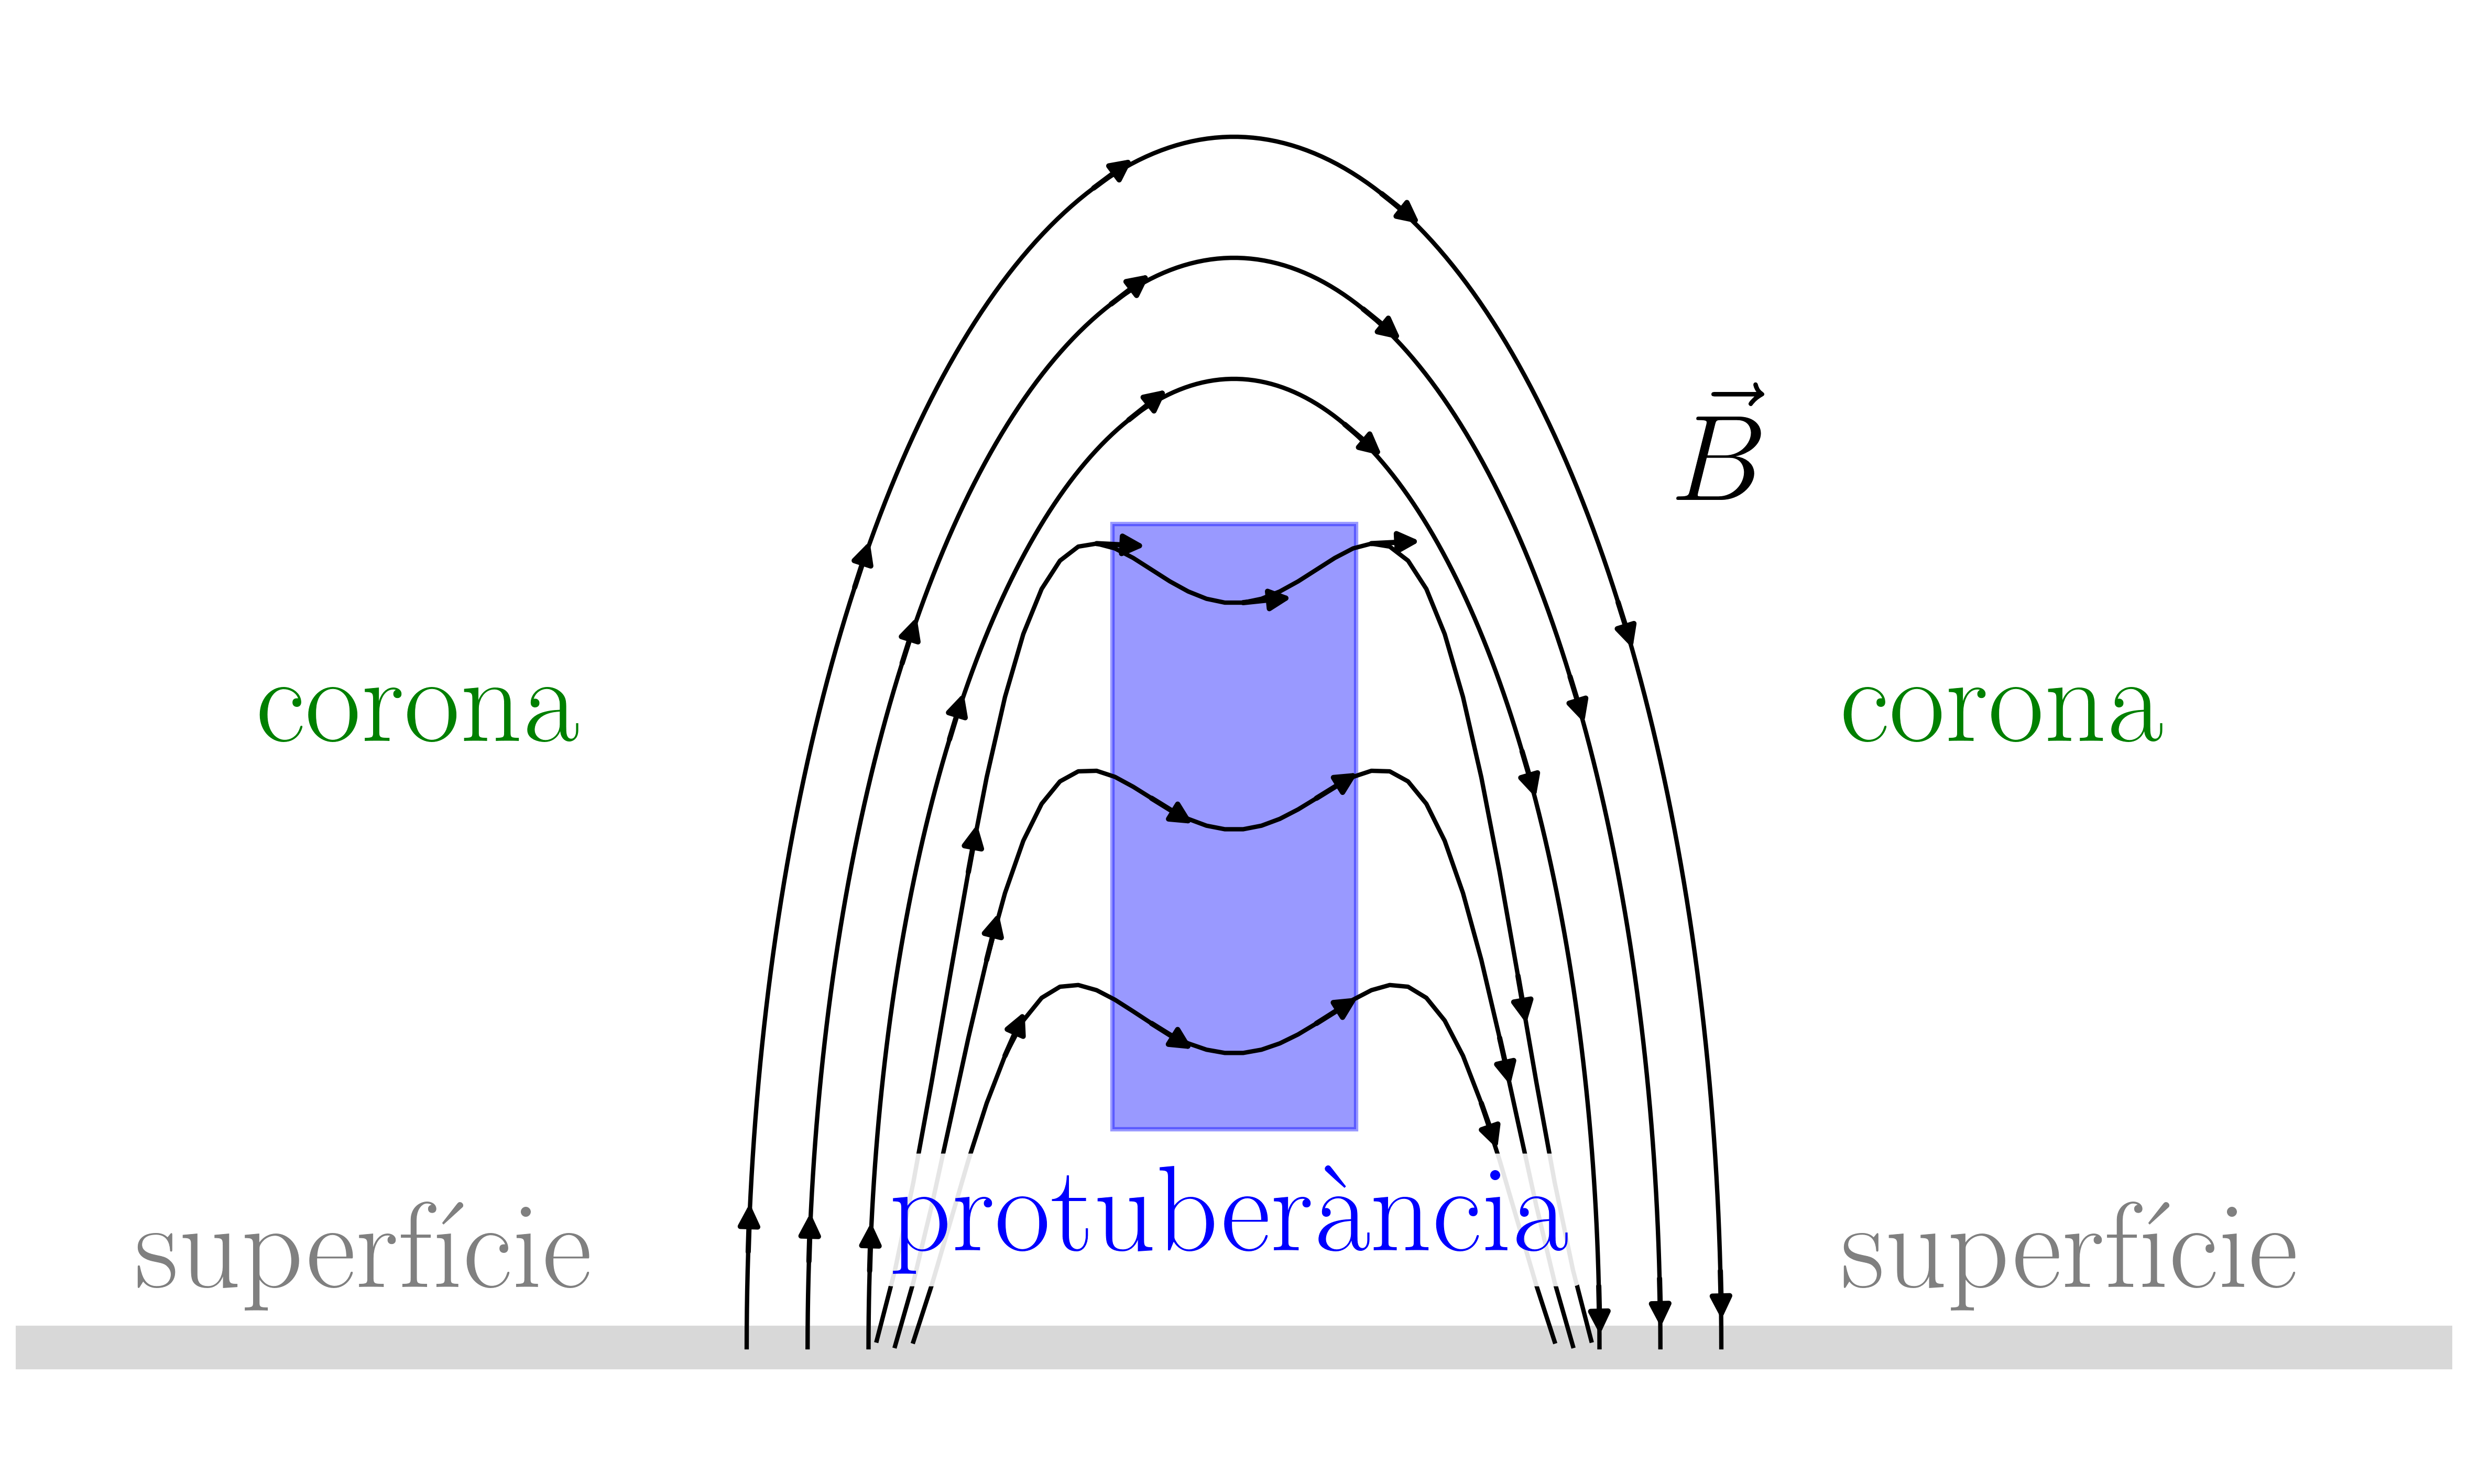
\includegraphics[width=\linewidth]{Representacions/prot_real.png}
        \caption{}
        \label{fig:prot_real}
    \end{subfigure}
    \hfill
    \begin{subfigure}{0.48\textwidth}
        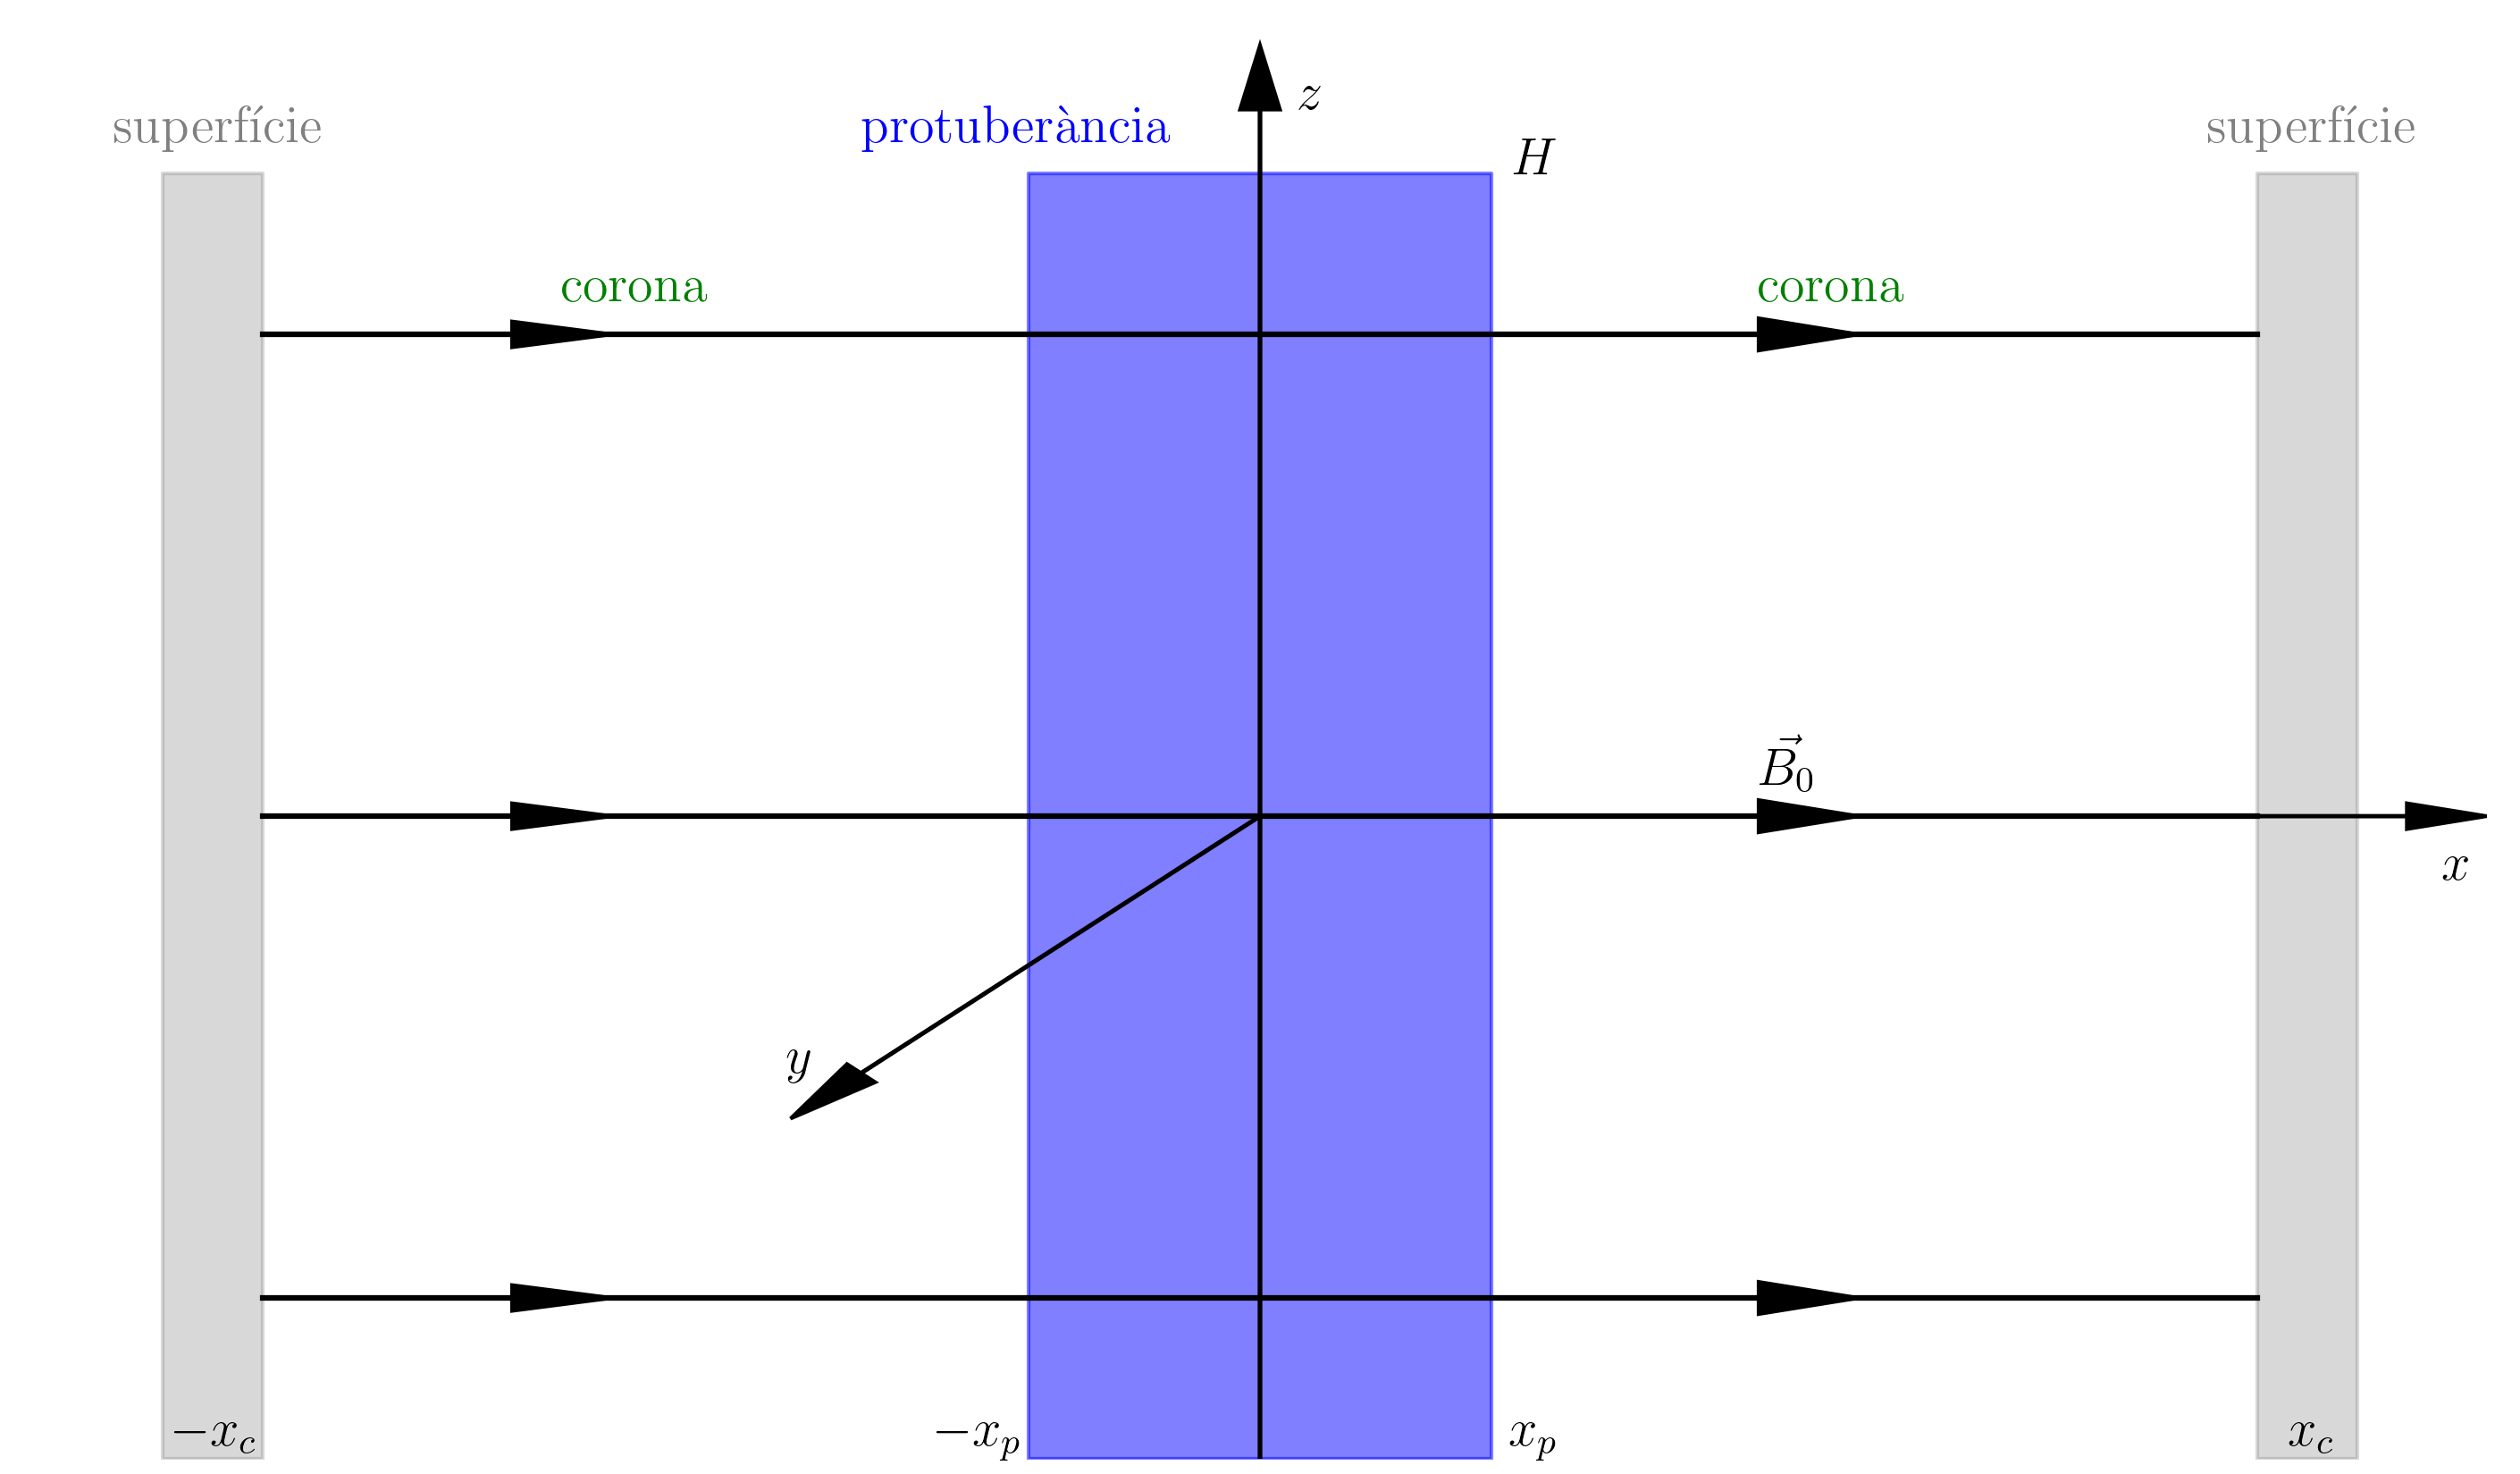
\includegraphics[width=\linewidth]{Representacions/protuberancia_solar_2d.png}
        \caption{}
        \label{fig:sistema}
    \end{subfigure}
    \caption{(a) Representació esquemàtica d'una protuberància solar en la corona.
    (b) Diagrama del sistema en equilibri tèrmic, com a làmina plana paral·lela a la superfície amb dimensions de $2x_p$ de gruix en direcció $\hat{x}$,
    d'alçada infinita en direcció $\hat{z}$ i infinita en direcció $\hat{y}$. El camp magnètic quiescent, $\bm{B}_{0}$, és horitzonal, en direcció $\hat{x}$.
    L'elecció dels eixos s'ha fet amb l'objectiu que la component del vector d'ona normal al camp magnètic estàtic sigui paral·lela a l'eix z.}
    %el vector d'ona sigui normal al camp magnètic estàtic i paral·lel a la direcció de la protuberància.
    \label{fig:protuberancia}
\end{figure}
\vspace{-10pt}
S'han fet altres consideracions que no afecten a les dimensions del sistema.
No obstant, juguen un paper clau com per exemple la condició d'adiabaticitat, que suposa l'inexistència d'intercanvi d'energia entre un element de plasma qualsevol i el seu entorn.
També es té en compte la diferència de densitats i temperatures en les tres zones, tot i que és la mateixa en les dues zones de la corona.
A més, s'ha de definir el sistema en equilibri termodinàmic (TD) i estàtic, per després pertorbar-lo lleugerament i comprovar la propagació d'aquesta pertorbació com a ona dins la protuberància i el medi.
S'ignoren els efectes gravitatoris i viscosos del plasma per simplificar encara més la situació.

El procediment seguit per obtenir els autovalors i les autofuncions dels modes normals, així com la relació de dispersió, és el següent.
Per començar es dedueixen les equacions MHD ideals (\hyperref[sec:equacionsMHD]{Sec.~2}) i es linealitzen suposant que les quantitats pertorbades es comporten com a ones
planes, ja que es tracta d'un medi uniforme en equilibri estàtic (\hyperref[subsec:linealització]{Subsec.~3.1}).
D'aquesta manera s'obté una relació de dispersió. Finalment s'adimensionalitzen les equacions per ser implementades en Dedalus (\hyperref[sec:mètode]{Sec.~4}).
